
\appendix
\renewcommand\thefigure{\thesection.\arabic{figure}} 
\setcounter{figure}{0} 
\section{Appendix - Suplementary figures}
%\section{Appendix A - Suplementary figures}


% multirater hypnogram
\begin{figure}[H]
    \centering
    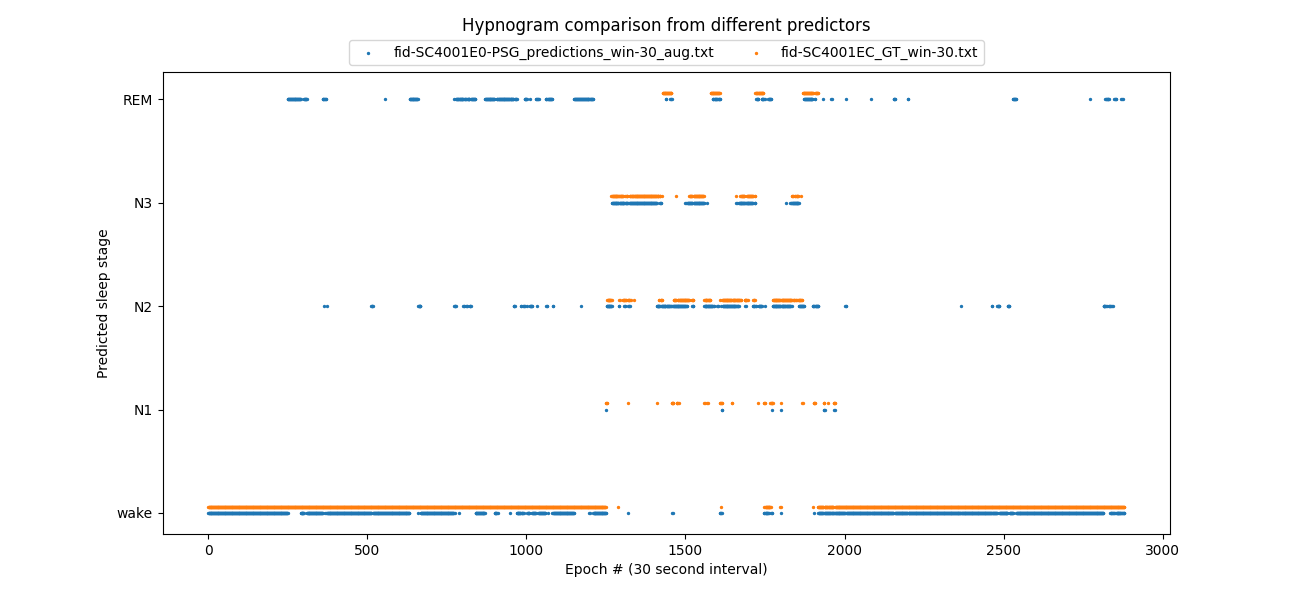
\includegraphics[width=0.99\linewidth]{Images/comparisonGT_hypnogramComparison.png}
    \vspace{-0.8em}
    \caption{Predicted (\texttt{...-PSG\_predictions\_...}, in blue) and ground truth (\texttt{...\_GT\_...}, in orange) hypnogram for sleep EDF database patient \#001}
    \label{fig:Appendix_GT_hypnogram}
\end{figure}



% CM for all predictions between 2 models
\begin{figure}[H]
    \centering
    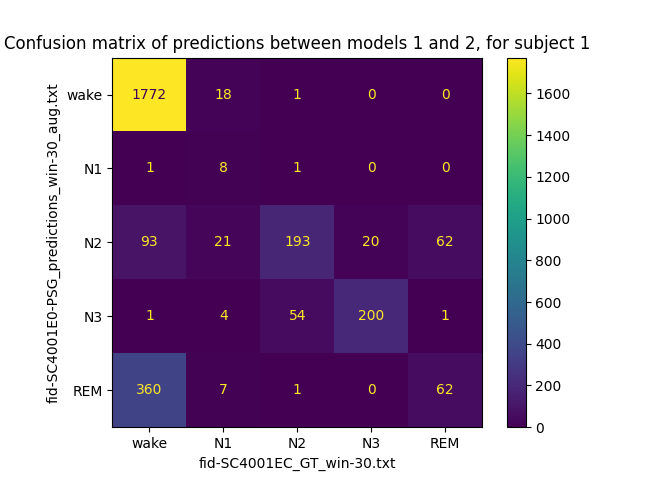
\includegraphics[width=0.6\linewidth]{Images/comparisonGT_predictionsCM.png}
    \vspace{-0.8em}
    %\caption{Probability of 1, 2 or 3 of the predictions agreeing for any time stamp}
    \caption{Confusion matrix for all epoch predictions between the predicted (\texttt{...-PSG\_predictions\_...}, across) and ground truth (\texttt{...\_GT\_...}, down) for sleep EDF database patient \#001}
    \label{fig:Appendix_GT_CM}
\end{figure}



% multirater hypnogram 2 subject
\begin{figure}[H]
    \centering
    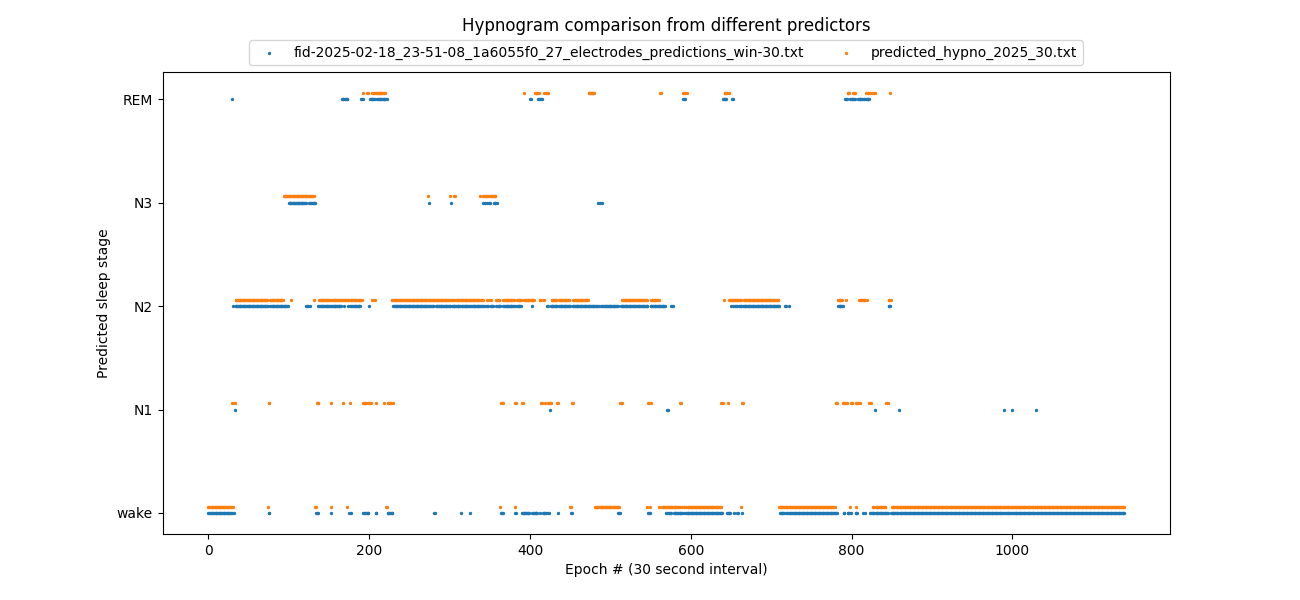
\includegraphics[width=0.99\linewidth]{Images/comparisson2_hypnogramComparison.png}
    \vspace{-0.8em}
    \caption{Multirater hypnogram comparison, with this pipeline's predictions (\texttt{fid\ ...\_predictions\_win-30...}, in blue) and Yasa's prediction (\texttt{predicted\_hypno\_2025}, in orange) hypnogram for subject \#2}
    \label{fig:Appendix_subj2_multirater_hypnogram}
\end{figure}

